\documentclass{article}

\usepackage[T1]{fontenc}
\usepackage[french]{babel}

\usepackage[letterpaper,top=2cm,bottom=2cm,left=3cm,right=3cm,marginparwidth=1.75cm]{geometry}

\usepackage{amsmath}
\usepackage{graphicx}
\usepackage[colorlinks=true, allcolors=blue]{hyperref}
\usepackage{eurosym}
\usepackage[group-separator={\ },output-decimal-marker={,}]{siunitx} 
\usepackage{amsfonts}
\usepackage{float}
\usepackage{pdflscape}
\usepackage{algorithm}
\usepackage{algorithmic}
\usepackage{array}
\usepackage{mdframed}
\usepackage{enumitem}
\usepackage{tcolorbox}
\usepackage{fontawesome5} % icônes
\usepackage{xcolor}
\usepackage{cancel} % trait diagonal pour barrer les expressions

\definecolor{lightgreen}{RGB}{230, 255, 230}

\newenvironment{conditions}
  {\par\vspace{\abovedisplayskip}\noindent\begin{tabular}{>{$}l<{$} @{${}={}$} l}}
  {\end{tabular}\par\vspace{\belowdisplayskip}}

\title{Impact de la fréquence de capitalisation sur le taux d'intérêt effectif et la valorisation des investissements}
\author{Gaëtan Bouget}

\begin{document}
\maketitle

\section{Problème}
Dans un contexte financier caractérisé par une diversification accrue des produits d’investissement, la variation des fréquences de capitalisation complique l’évaluation objective des rendements réels. Ainsi, deux actifs affichant un même taux nominal annuel peuvent générer des rendements distincts en raison des différentes fréquences de capitalisation, amplifiant ainsi l'effet des intérêts composés.

\section{Objectif}
L'objectif consiste à fournir une compréhension approfondie des mécanismes influençant le rendement réel des investissements et à établir une base solide pour la comparaison de diverses stratégies financières.

\section{Méthode}
L'approche adoptée pour atteindre l'objectif se décline en quatre étapes :
\begin{enumerate}
	\item calcul du capital final pour les actifs à intérêts simples ;
	\item prise en compte des intérêts composés dans l’analyse comparative ;
	\item démonstration de la supériorité des intérêts composés par développement binomial ;
	\item établissement de la formule du taux effectif annuel (TEA).
\end{enumerate}

Afin de faciliter les applications numériques avant de généraliser, l'analyse se concentre sur l'investissement d'un capital initial de \( C_0 = 100\,000\ \text{€} \), réparti sur quatre actifs décrits dans le tableau~\ref{tab:scenarios}.

\begin{table}[h!]
	\centering
	\begin{tabular}{|c|c|c|c|}
		\hline
		\textbf{Actif} & \textbf{Type d'intérêt} & \textbf{Fréquence de capitalisation} & \textbf{Taux périodique}                \\
		\hline
		\(A_q^s\)      & Intérêts simples        & Quotidienne                           & \(r_\text{quotidien} = \frac{5}{365}\%\) \\
		\hline
		\(A_a^s\)      & Intérêts simples        & Annuelle                              & \(r_\text{annuel} = 5\%\)                \\
		\hline
		\(A_q^c\)      & Intérêts composés      & Quotidienne                           & \(r_\text{quotidien} = \frac{5}{365}\%\) \\
		\hline
		\(A_a^c\)      & Intérêts composés      & Annuelle                              & \(r_\text{annuel} = 5\%\)                \\
		\hline
	\end{tabular}
	\caption{Scénarios d'investissement avec un capital initial \(C_0 = 100\,000\ \text{€}\).}
	\label{tab:scenarios}
\end{table}

Chaque étape est constituée d'une série de questions pour progresser pas à pas.

\subsection{Hypothèses de travail}
Les conditions suivantes sont posées :
\begin{itemize}
	\item Les intérêts sont calculés selon la fréquence de capitalisation définie pour chaque actif. Aucune capitalisation intermédiaire ni prorata temporis ne s'applique en cas de retrait avant la fin de la période de capitalisation.
	\item Une année est considérée comme comprenant 365 jours.
	\item Aucun frais ni taxe n'est appliqué.
	\item Aucun versement ou retrait supplémentaire n’est effectué durant la période d'investissement (seul le capital initial \( C_0 \) est investi).
	\item Le taux de rendement est constant dans le temps.
\end{itemize}

\subsection{Questions}
\subsubsection*{Étape 1 : calcul du capital final pour les actifs à intérêts simples}

\begin{tcolorbox}[
		colback=lightgreen, 
		colframe=lightgreen, 
		boxrule=0.5pt, 
		arc=0pt, 
		left=10pt, 
		right=10pt, 
		top=6pt, 
		bottom=6pt, 
		boxsep=2pt, 
		before upper={\faLightbulb\hspace{10pt}}
	]
	Les intérêts simples sont calculés uniquement sur le capital initial, et le montant des intérêts gagnés chaque période est constant. La formule suivante reflète bien cette caractéristique, car le produit \( r \times t \) est simplement ajouté au capital initial :
	
	\[
		C^{\text{simple}}(t) = C_0 \left(1 + r \times t\right)
	\]
	    
	où :
	\begin{itemize}
		\item \( C^{\text{simple}}(t) \) est le capital accumulé après une période \( t \).
		\item \( C_0 \) est le capital initial investi.
		\item \( r \) est le taux d'intérêt nominal (exprimé sous forme décimale, par exemple, 5\% devient $\frac{5}{100}$ soit 0,05).
		\item \( t \) est le temps écoulé, qui peut être exprimé en années ou en jours, selon la fréquence de capitalisation.
	\end{itemize}
\end{tcolorbox}

\begin{enumerate}[label=\textbf{Q1.\arabic*}]
	\item Soit un capital initial \( C_0 = 100\,000\ \text{€} \) investi, calculer le capital final de l'actif \( A_q^s \) après une durée \( t \) égale à :
	      \begin{enumerate}[label=(\alph*)]
	      	\item \( t = 1 \) jour
	      	\item \( t = 30 \) jours
	      	\item \( t = 1 \) an
	      	\item \( t = 30 \) ans
	      \end{enumerate}
	      
	\item Soit un capital initial \( C_0 = 100\,000\ \text{€} \) investi, calculer le capital final de l'actif \( A_a^s \) après une durée \( t \) égale à :
	      \begin{enumerate}[label=(\alph*)]
	      	\item \( t = 1 \) jour
	      	\item \( t = 30 \) jours
	      	\item \( t = 1 \) an
	      	\item \( t = 30 \) ans
	      \end{enumerate}
	          
	\item Remplir le tableau suivant en calculant les capitaux finaux pour les deux types d'actifs à différents horizons de temps :\\
	      \begin{table}[h!]
	      	\centering
	      	\begin{tabular}{|c|c|c|c|c|}
	      		\hline
	      		\textbf{Actif} & \textbf{1 jour} & \textbf{30 jours} & \textbf{1 an} & \textbf{30 ans} \\
	      		\hline
	      		\( A_q^s \)    &                 &                   &               &                 \\
	      		\hline
	      		\( A_a^s \)    &                 &                   &               &                 \\
	      		\hline
	      	\end{tabular}
	      	\caption{Capital final pour différentes durées d'investissement avec intérêts simples et un capital initial de \( C_0 = 100\,000\ \text{€} \).}
	      	\label{tab:simple_interest_results}
	      \end{table}
	      
	\item Soit un capital initial \( C_0 \) et un taux nominal annuel \( r_a \) ou un taux nominal quotidien \( r_q \), exprimer les fonctions permettant de calculer le capital final en fonction de la durée d'investissement \( t \) (exprimée en jours) pour chacun des deux actifs à intérêts simples :
	      \begin{enumerate}[label=(\alph*)]
	      	\item \( C^s_q(t) \) pour un actif à capitalisation quotidienne avec un taux périodique \( r_q \) ;
	      	\item \( C^s_a(t) \) pour un actif à capitalisation annuelle avec un taux \( r_a \).
	      \end{enumerate}
	      
	\item Tracer les courbes \( C^s_q(t) \) et \( C^s_a(t) \) pour \( C_0 \in \{50\,000, 100\,000, 200\,000\} \, \text{€} \). La durée \( t \) (en abscisse) varie de 0 à 40 ans. Commenter l'évolution du capital dans le temps en fonction des différents montants de capital initial.
	      
	\item Pour les trois valeurs de capital initial \( C_0 \in \{50\,000, 100\,000, 200\,000\} \)~€, déterminer graphiquement le capital final obtenu pour des durées d'investissement \( t \) égales à 10 ans, 20 ans et 30 ans. Quel est le coefficient multiplicateur du capital initial en fonction de ces durées ?
	      
	\item Exprimer le coefficient multiplicateur \( k(t) \) du capital initial en fonction de la durée d'investissement \( t \) et du taux périodique \( r \). Vérifier la cohérence des résultats avec ceux obtenus graphiquement en appliquant la formule pour un taux de 5\,\% et des durées de 10, 20 et 30 ans.
	      
	\item Représenter graphiquement le coefficient multiplicateur du capital initial en fonction de la durée d'investissement pour le taux périodique $r_q = 5\%$. Relever graphiquement le coefficient multiplicateur pour les durées d'investissement à 10 ans, 20 ans, 30 ans, 50 ans et 100 ans.
	      
	\item Utiliser les valeurs du coefficient multiplicateur obtenues graphiquement pour déterminer le capital final après 10 ans, 20 ans, 30 ans, 50 ans et 100 ans, en partant d'un capital initial de $72\,924,56$\ € et avec un taux périodique de 5\%.
	      
	\item Calculer le coefficient directeur des droites \( C^s_q \) avec \( C_0 \in \{50\,000, 100\,000, 200\,000\} \)~€ en utilisant les points d'abscisse suivants :
	      \begin{itemize}
	      	\item \( x_a = 0 \) et \( x_b = 1 \) ;
	      	\item \( x_a = 32 \) et \( x_b = 1\,946 \) ;
	      	\item \( x_a = 364\,999 \) et \( x_b = 365\,000 \).
	      \end{itemize}
	      \begin{tcolorbox}[
	      		colback=lightgreen,
	      		colframe=lightgreen,
	      		boxrule=0.5pt,
	      		arc=0pt,
	      		left=10pt,
	      		right=10pt,
	      		top=6pt,
	      		bottom=6pt,
	      		boxsep=2pt,
	      		before upper={\faLightbulb\hspace{10pt}}
	      	]
	      	La pente d'une droite, également appelée coefficient directeur, mesure la variation verticale (changement en \( y \)) par rapport à la variation horizontale (changement en \( x \)). Elle indique la direction et l'inclinaison de la droite.
	      	    
	      	\textbf{Formule générale :}
	      	    
	      	\[
	      		m = \frac{\Delta y}{\Delta x} = \frac{C(x_b) - C(x_a)}{x_b - x_a}\,,
	      	\]
	      	    
	      	où \( m \) est le coefficient directeur, \( C(x_a) \) et \( C(x_b) \) sont les valeurs de la fonction \( C \) aux points \( x_a \) et \( x_b \), respectivement.
	      \end{tcolorbox}
	      
	\item Interpréter financièrement le coefficient directeur.
	      
	\item À partir de la formule générale du coefficient directeur, expliquer comment la pente \( m \) de la fonction \( C_q^s(t) = C_0 \times \left(1 + \frac{0{,}05}{365} \times t\right) \) peut être simplifiée pour obtenir l'expression \( m = C_0 \times r \), où \( r \) est le rendement périodique quotidien, soit \( r = \frac{0{,}05}{365} \).
	      
	\item Quelle est la signification du caractère constant du coefficient directeur dans le cas des intérêts simples ?
	      
	\item Donner quelques exemples de situations de la vie courante où les intérêts sont simples.
	      
	\item Quel est l'effet de l'inflation et de la déflation sur le rendement ? Prendre en compte l'objectif de la Banque Centrale Européenne (BCE).
	      
	\item Que se passe-t-il si les intérêts perçus sont réinvestis dans un actif financier ?
	      
	      
	      % ================================================================================
	      % ================================================================================
	      \subsection*{Étape 2 : ajout des actifs à intérêts composés au comparatif}
	      % ================================================================================
	      \begin{tcolorbox}[
	      		colback=lightgreen, 
	      		colframe=lightgreen, 
	      		boxrule=0.5pt, 
	      		arc=0pt, 
	      		left=10pt, 
	      		right=10pt, 
	      		top=6pt, 
	      		bottom=6pt, 
	      		boxsep=2pt, 
	      		before upper={\faLightbulb\hspace{10pt}}
	      	]
	      	Les intérêts composés sont calculés sur le capital initial, auquel s'ajoutent progressivement les intérêts accumulés :
	      	    
	      	
	      	\[
	      		C^{\text{composé}}(t) = C_0 \times (1 + r)^t
	      	\]
	      	    
	      	où :
	      	\begin{itemize}
	      		\item \( C^{\text{composé}}(t) \) est le capital accumulé après une période \( t \).
	      		\item \( C_0 \) est le capital initial investi.
	      		\item \( r \) est le taux d'intérêt nominal (exprimé sous forme décimale, par exemple, 5\% devient $\frac{5}{100}$ soit 0,05).
	      		\item \( t \) est le temps écoulé, exprimé en années ou en jours, selon la fréquence de capitalisation.
	      	\end{itemize}
	      \end{tcolorbox}
	      
	      \begin{tcolorbox}[
	      		colback=lightgreen, 
	      		colframe=lightgreen, 
	      		boxrule=0.5pt, 
	      		arc=0pt, 
	      		left=10pt, 
	      		right=10pt, 
	      		top=6pt, 
	      		bottom=6pt, 
	      		boxsep=2pt, 
	      		before upper={\faLightbulb\hspace{10pt}}
	      	]
	      	Le calcul des intérêts composés est modélisé par une fonction exponentielle, notée sous la forme $f(x)=a^x$, où $a$ est une constante positive et $x$ correspond au temps ou au nombre de périodes de capitalisation.
	      	
	      	À l'inverse, une fonction puissance, exprimée par $f(x)=x^a$, caractérise une croissance polynomiale. La fonction exponentielle surpasse en vitesse la fonction puissance, ce qui met en évidence le phénomène d'effet boule de neige des intérêts composés : les intérêts générés à chaque période s'ajoutent au capital, accélérant ainsi son expansion au cours du temps.
	      	
	      	Moyen mnémotechnique : 
	      	\begin{itemize}
	      		\item Fonction \underline{expo}nent\underline{ie}l\underline{le} = l'\underline{expo}sant var\underline{ie}, la croissance s'embal\underline{le}.
	      		\item Fonction puiss\underline{an}ce = la puissance est const\underline{an}te.
	      	\end{itemize}
	      \end{tcolorbox}
	      
	      \begin{enumerate}[label=\textbf{Q2.\arabic*}]
	      	\item Soit un capital initial \( C_0 = 100\,000\ \text{€} \) investi, calculer le capital final de l'actif \( A_q^c \) après une durée \( t \) égale à :
	      	      \begin{enumerate}[label=(\alph*)]
	      	      	\item \( t = 1 \) jour
	      	      	\item \( t = 30 \) jours
	      	      	\item \( t = 1 \) an
	      	      	\item \( t = 30 \) ans
	      	      \end{enumerate}
	      	          
	      	\item Soit un capital initial \( C_0 = 100\,000\ \text{€} \) investi, calculer le capital final de l'actif \( A_a^q \) après une durée \( t \) égale à :
	      	      \begin{enumerate}[label=(\alph*)]
	      	      	\item \( t = 1 \) jour
	      	      	\item \( t = 30 \) jours
	      	      	\item \( t = 1 \) an
	      	      	\item \( t = 30 \) ans
	      	      \end{enumerate}
	      	      
	      	      
	      	\item Remplir le tableau suivant en calculant les capitaux finaux pour les deux types d'actifs à différents horizons de temps :\\
	      	      \begin{table}[h!]
	      	      	\centering
	      	      	\begin{tabular}{|c|c|c|c|c|}
	      	      		\hline
	      	      		\textbf{Actif} & \textbf{1 jour} & \textbf{30 jours} & \textbf{1 an} & \textbf{30 ans} \\
	      	      		\hline
	      	      		\( A_q^s \)    &                 &                   &               &                 \\
	      	      		\hline
	      	      		\( A_a^s \)    &                 &                   &               &                 \\
	      	      		\hline
	      	      		\( A_q^c \)    &                 &                   &               &                 \\
	      	      		\hline
	      	      		\( A_a^c \)    &                 &                   &               &                 \\
	      	      		\hline
	      	      	\end{tabular}
	      	      	\caption{Capital final pour différentes durées d'investissement avec intérêts composés et un capital initial de \( C_0 = 100\,000\ \text{€} \).}
	      	      	\label{tab:simple_interest_results}
	      	      \end{table}
	      	      
	      	\item Soit un capital initial \( C_0 \) et un taux nominal annuel \( r_a \) ou un taux nominal quotidien \( r_q \), exprimer les fonctions permettant de calculer le capital final en fonction de la durée d'investissement \( t \) (exprimée en jours) pour chacun des deux actifs à intérêts composés :
	      	      \begin{enumerate}[label=(\alph*)]
	      	      	\item \( C^c_q(t) \) pour un actif à capitalisation quotidienne avec un taux périodique \( r_q \) ;
	      	      	\item \( C^c_a(t) \) pour un actif à capitalisation annuelle avec un taux \( r_a \).
	      	      \end{enumerate}
	      	          
	      	\item Sur le graphique des courbes $C^s_q$ et $C^s_q$, ajouter le tracé de \( C^c_q(t) \) et \( C^c_a(t) \) pour \( C_0 \in \{50\,000, 100\,000, 200\,000\} \, \text{€} \). La durée \( t \) (en abscisse) varie de 0 à 40 ans. Commenter l'évolution du capital dans le temps en fonction des différents montants de capital initial et du type d'actif.
	      	          
	      	\item Pour les trois valeurs de capital initial \( C_0 \in \{50\,000, 100\,000, 200\,000\} \)~€, déterminer graphiquement le capital final obtenu pour des durées d'investissement \( t \) égales à 10 ans, 20 ans et 30 ans. Quel est le coefficient multiplicateur du capital initial en fonction de ces durées ?
	      \end{enumerate}
	      
\end{enumerate}

\newpage
\section{Solution}
\subsection*{Étape 1 : calcul du capital final pour les actifs à intérêts simples}

\noindent
\textbf{Formule générale pour les intérêts simples :}
\[
	C(t) = C_0 \times \left(1 + r \times t\right)
\]
où $r_a = 5\% = 0,05$ et \( r_q = \frac{5}{365}\% = \frac{0,05}{365} \), et \( t \) la durée exprimée en jours.

\begin{enumerate}[label=\textbf{R1.\arabic*}]
	\item \textbf{Actif \( A_q^s \) (capitalisation quotidienne avec intérêts simples)}
	      \[
	      	C_q^s(t) = 100\,000 \times \left(1 + \frac{0,05}{365} \times t\right)
	      \]
	      \begin{enumerate}[label=(\alph*)]
	      	\item \( t = 1 \) jour : 
	      	      \[
	      	      	C_q^s(1) = 100\,000 \times \left(1 + \frac{0,05}{365} \times 1\right) = \boxed{100\,013,70\ \text{€}}
	      	      \]
	      	              
	      	\item $t = 30$ jours : 
	      	      \[
	      	      	C_q^s(30) = 100\,000 \times \left(1 + \frac{0,05}{365} \times 30\right) = \boxed{100\,410,96\ \text{€}}
	      	      \]
	      	              
	      	\item $t = 1\ \text{an} = 365\ \text{jours}$~: 
	      	      \begin{align*}
	      	      	C_q^s(365) & = 100\,000 \times \left(1 + \frac{0,05}{365} \times 365\right) \\
	      	      	           & = 100\,000 \times (1 + 0,05)                                   \\
	      	      	           & = 100\,000 \times 1,05                                         \\
	      	      	           & = \boxed{105\,000,00\ \text{€}}                              
	      	      \end{align*}
	      	              
	      	\item $t = 30\ \text{ans} = 10\,950\ \text{jours}$~: 
	      	      \begin{align*}
	      	      	C_q^s(10\,950) & = 100\,000 \times \left(1 + \frac{0,05}{365} \times 10\,950\right) \\
	      	      	               & = 100\,000 \times (1 + 1,5)                                        \\
	      	      	               & = 100\,000 \times 2,5                                              \\
	      	      	               & = \boxed{250\,000,00\ \text{€}}                                  
	      	      \end{align*}
	      	              
	      \end{enumerate}
	      
	\item \textbf{Actif \( A_a^s \) (capitalisation annuelle avec intérêts simples)} \\
	      Puisque les intérêts ne sont ajoutés que si le capital reste investi pendant une année complète (365 jours), la fonction \emph{partie entière}, notée $\lfloor \cdot \rfloor$, est utilisée pour modéliser cette condition.
	      \[
	      	C_a^s(t) = 100\,000 \times \left(1 + 0,05 \times \left\lfloor \frac{t}{365} \right\rfloor \right)
	      \]
	      \begin{enumerate}[label=(\alph*)]
	      	\item \( t = 1 \) jour : 
	      	      \begin{align*}
	      	      	C_a^s(1) & = 100\,000 \times \left(1 + 0,05 \times \left\lfloor \frac{1}{365} \right\rfloor \right) \\
	      	      	         & = 100\,000 \times \left(1 + 0,05 \times 0 \right)                                        \\
	      	      	         & = 100\,000 \times (1 + 0)                                                                \\
	      	      	         & = 100\,000 \times 1                                                                      \\
	      	      	         & = \boxed{100\,000\ \text{€}}                                                           
	      	      \end{align*}
	      	              
	      	\item \( t = 30 \) jours : 
	      	      \begin{align*}
	      	      	C_a^s(30) & = 100\,000 \times \left(1 + 0,05 \times \left\lfloor \frac{30}{365} \right\rfloor \right) \\
	      	      	          & = 100\,000 \times \left(1 + 0,05 \times 0 \right)                                         \\
	      	      	          & = \boxed{100\,000\ \text{€}}                                                            
	      	      \end{align*}
	      	              
	      	\item $t = 1\ \text{an} = 365\ \text{jours}$~: 
	      	      \begin{align*}
	      	      	C_a^s(365) & = 100\,000 \times \left(1 + 0,05 \times \left\lfloor \frac{365}{365} \right\rfloor \right) \\
	      	      	           & = 100\,000 \times \left(1 + 0,05 \times 1 \right)                                          \\
	      	      	           & = 100\,000 \times \left(1 + 0,05 \right)                                                   \\
	      	      	           & = 100\,000 \times 1,05                                                                     \\
	      	      	           & = \boxed{105\,000\ \text{€}}                                                             
	      	      \end{align*}
	      	              
	      	\item $t = 30\ \text{ans} = 10\,950\ \text{jours}$~: 
	      	      \begin{align*}
	      	      	C_a^s(10\,950) & = 100\,000 \times \left(1 + 0,05 \times \left\lfloor \frac{10\,950}{365} \right\rfloor \right) \\
	      	      	               & = 100\,000 \times \left(1 + 0,05 \times 30 \right)                                             \\
	      	      	               & = 100\,000 \times \left(1 + 1,5 \right)                                                        \\
	      	      	               & = 100\,000 \times 2,5                                                                          \\
	      	      	               & = \boxed{205\,000\ \text{€}}                                                                 
	      	      \end{align*}
	      \end{enumerate}
	      
	\item Voir table \ref{tab:simple_interest_results}.
	      \begin{table}[h!]
	      	\centering
	      	\begin{tabular}{|c|c|c|c|c|}
	      		\hline
	      		\textbf{Actif} & \textbf{1 jour}  & \textbf{30 jours} & \textbf{1 an}    & \textbf{30 ans}  \\
	      		\hline
	      		\( A_q^s \)    & 100\,013,70\ € & 100\,410,96\ €  & 105\,000,00\ € & 250\,000,00\ € \\
	      		\hline
	      		\( A_a^s \)    & 100\,000,00\ € & 100\,000,00\ €  & 105\,000,00\ € & 250\,000,00\ € \\
	      		\hline
	      	\end{tabular}
	      	\caption{Résultats pour les intérêts simples (\( C_0 = 100\,000\ \text{€} \)).}
	      	\label{tab:simple_interest_results}
	      \end{table}
	      
	\item \textbf{Fonctions de capitalisation} :
	      \begin{enumerate}[label=(\alph*)]
	      	\item \( C_q^s(t) = C_0 \times \left(1 + r_q \times t\right) \)
	      	\item \( C_a^s(t) = C_0 \times \left(1 + r_a \times \left\lfloor\frac{t}{365}\right\rfloor\right) \)
	      \end{enumerate}
	      
	\item Le graphique en figure \ref{fig:interets_simples} représente six courbes correspondant aux fonctions :
	      \[
	      	C_q^s(t) = C_0 \times \left(1 + \frac{0{,}05}{365} \times t\right)
	      \]
	      et
	      \[
	      	\begin{aligned}
	      		C_a^s(t) & = C_0 \times \left(1 + 0{,}05 \times \left\lfloor\frac{t}{365}\right\rfloor\right) \\
	      		         & = C_0 \times \left(1 + 0{,}05 \times \frac{t - (t \!\!\!\mod 365)}{365}\right),    
	      	\end{aligned}
	      \]
	      avec \( C_0 \in \bigl\{50\,000,\ 100\,000,\ 200\,000\bigr\}\,\text{€} \).
	      
	      Axes :
	      \begin{itemize}
	      	\item L'axe des abscisses (horizontal) représente la durée en jours.
	      	\item L'axe des ordonnées (vertical) représente le capital en euros.
	      \end{itemize}
	      
	      Comparaison :
	      \begin{itemize}
	      	\item Les courbes de capitalisation quotidienne $C_q^s(t)$ montrent une croissance linéaire continue.
	      	\item Les courbes de capitalisation annuelle $C_a^s(t)$ présentent une fonction en escalier avec des sauts discrets à chaque année, où chaque saut suit une croissance linéaire, reflétant une augmentation constante et régulière du capital.
	      	\item Lorsqu'une année est révolue, les deux types de capitalisation convergent, car les intérêts annuels sont ajoutés.
	      \end{itemize}
	      
	      \begin{figure}[h!]
	      	\centering
	      	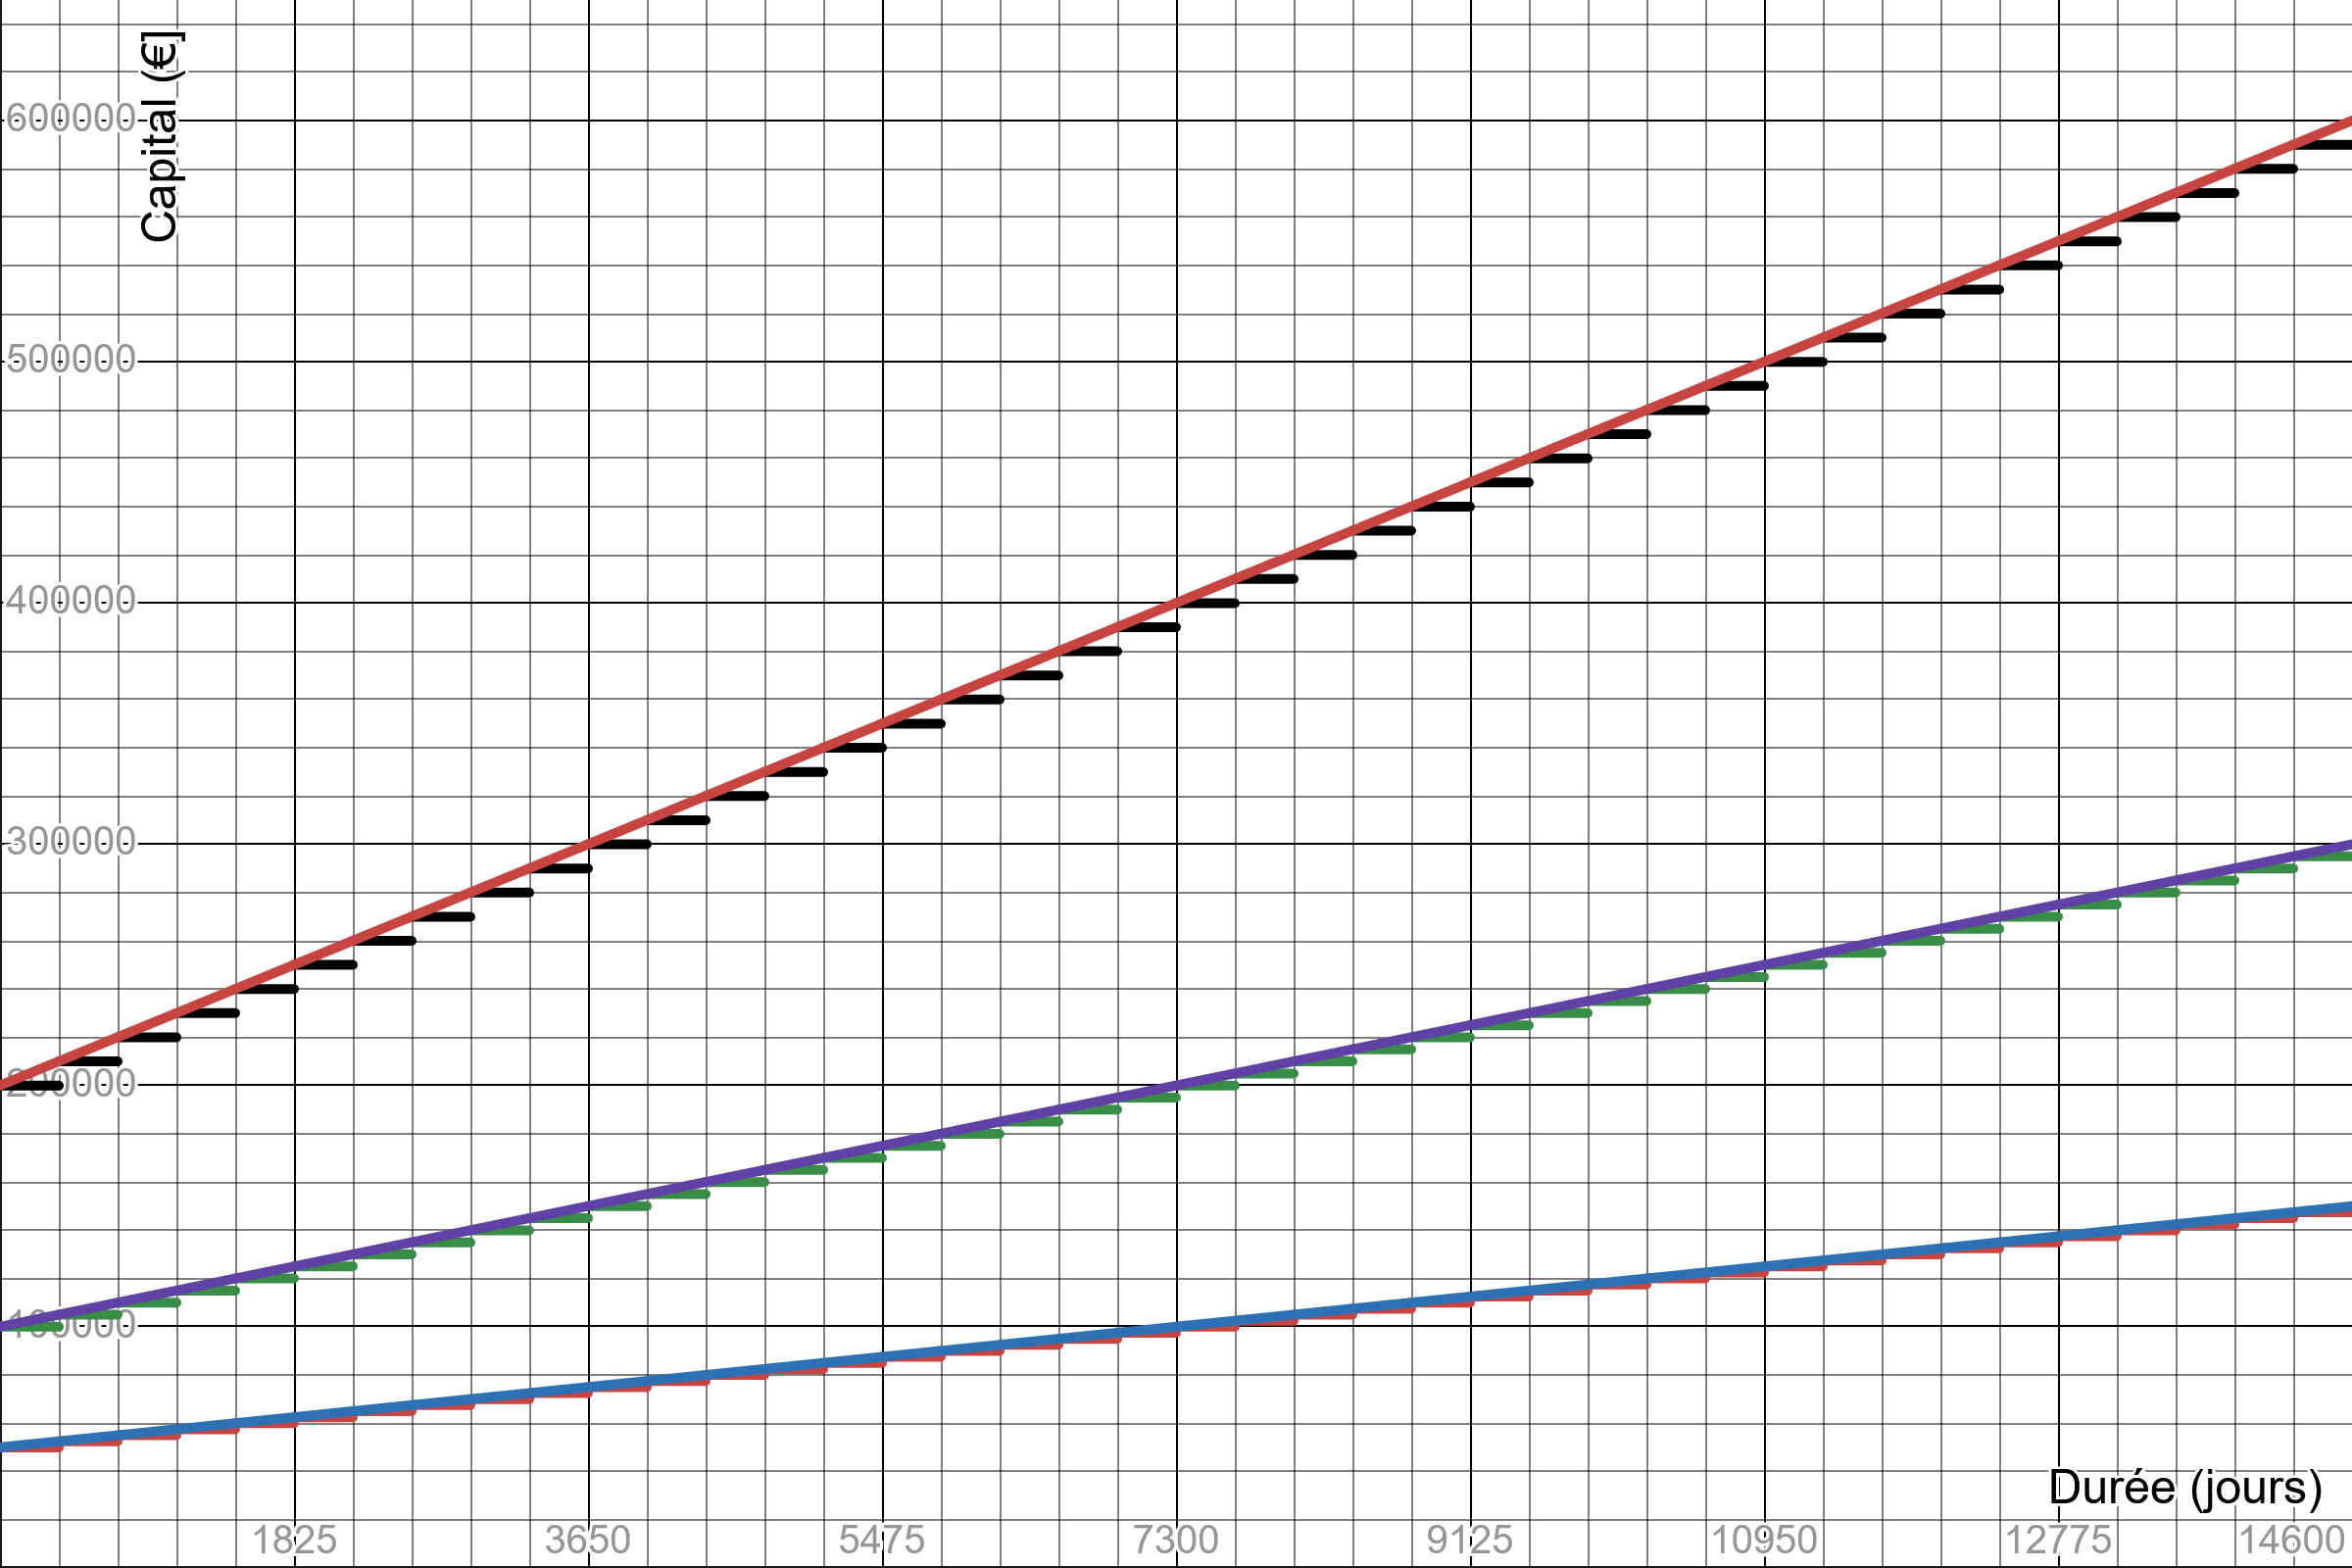
\includegraphics[width=\textwidth]{interets_simples.png}
	      	\caption{Comparaison de la capitalisation quotidienne et annuelle des intérêts simples.}
	      	\label{fig:interets_simples}
	      \end{figure}
	      
	\item Le capital final est lu graphiquement sur la figure \ref{fig:lecture_graphique_interets_simples}:
	      \begin{align*}
	      	\begin{array}{rcl}
	      	50\,000\,\text{€}  & \xrightarrow{\text{10 ans}} & 75\,000\,\text{€} \\
	      	100\,000\,\text{€} & \xrightarrow{\text{10 ans}} & 150\,000\,\text{€} \\
	      	200\,000\,\text{€} & \xrightarrow{\text{10 ans}} & 300\,000\,\text{€} \\
	      	50\,000\,\text{€}  & \xrightarrow{\text{20 ans}} & 100\,000\,\text{€} \\
	      	100\,000\,\text{€} & \xrightarrow{\text{20 ans}} & 200\,000\,\text{€} \\
	      	200\,000\,\text{€} & \xrightarrow{\text{20 ans}} & 400\,000\,\text{€} \\
	      	50\,000\,\text{€}  & \xrightarrow{\text{30 ans}} & 125\,000\,\text{€} \\
	      	100\,000\,\text{€} & \xrightarrow{\text{30 ans}} & 250\,000\,\text{€} \\
	      	200\,000\,\text{€} & \xrightarrow{\text{30 ans}} & 500\,000\,\text{€}
	      	\end{array}
	      	\qquad
	      	\begin{array}{rrcl}
	      	10 \text{ ans :} & \displaystyle \frac{75\,000}{50\,000}  & = \displaystyle \frac{150\,000}{100\,000} & = \displaystyle \frac{300\,000}{200\,000} = 1,5 \\[1em]
	      	20 \text{ ans :} & \displaystyle \frac{100\,000}{50\,000} & = \displaystyle \frac{200\,000}{100\,000} & = \displaystyle \frac{400\,000}{200\,000} = 2   \\[1em]
	      	30 \text{ ans :} & \displaystyle \frac{125\,000}{50\,000} & = \displaystyle \frac{250\,000}{100\,000} & = \displaystyle \frac{500\,000}{200\,000} = 2,5 
	      	\end{array}
	      \end{align*}
	      
	      \begin{itemize}
	      	\item Le capital initial est multiplié par 1,5 après 10 ans.
	      	\item Le capital initial est multiplié par 2 après 20 ans.
	      	\item Le capital initial est multiplié par 2,5 après 30 ans.
	      \end{itemize}
	          
	      \begin{figure}[h!]
	      	\centering
	      	\makebox[\textwidth][c]{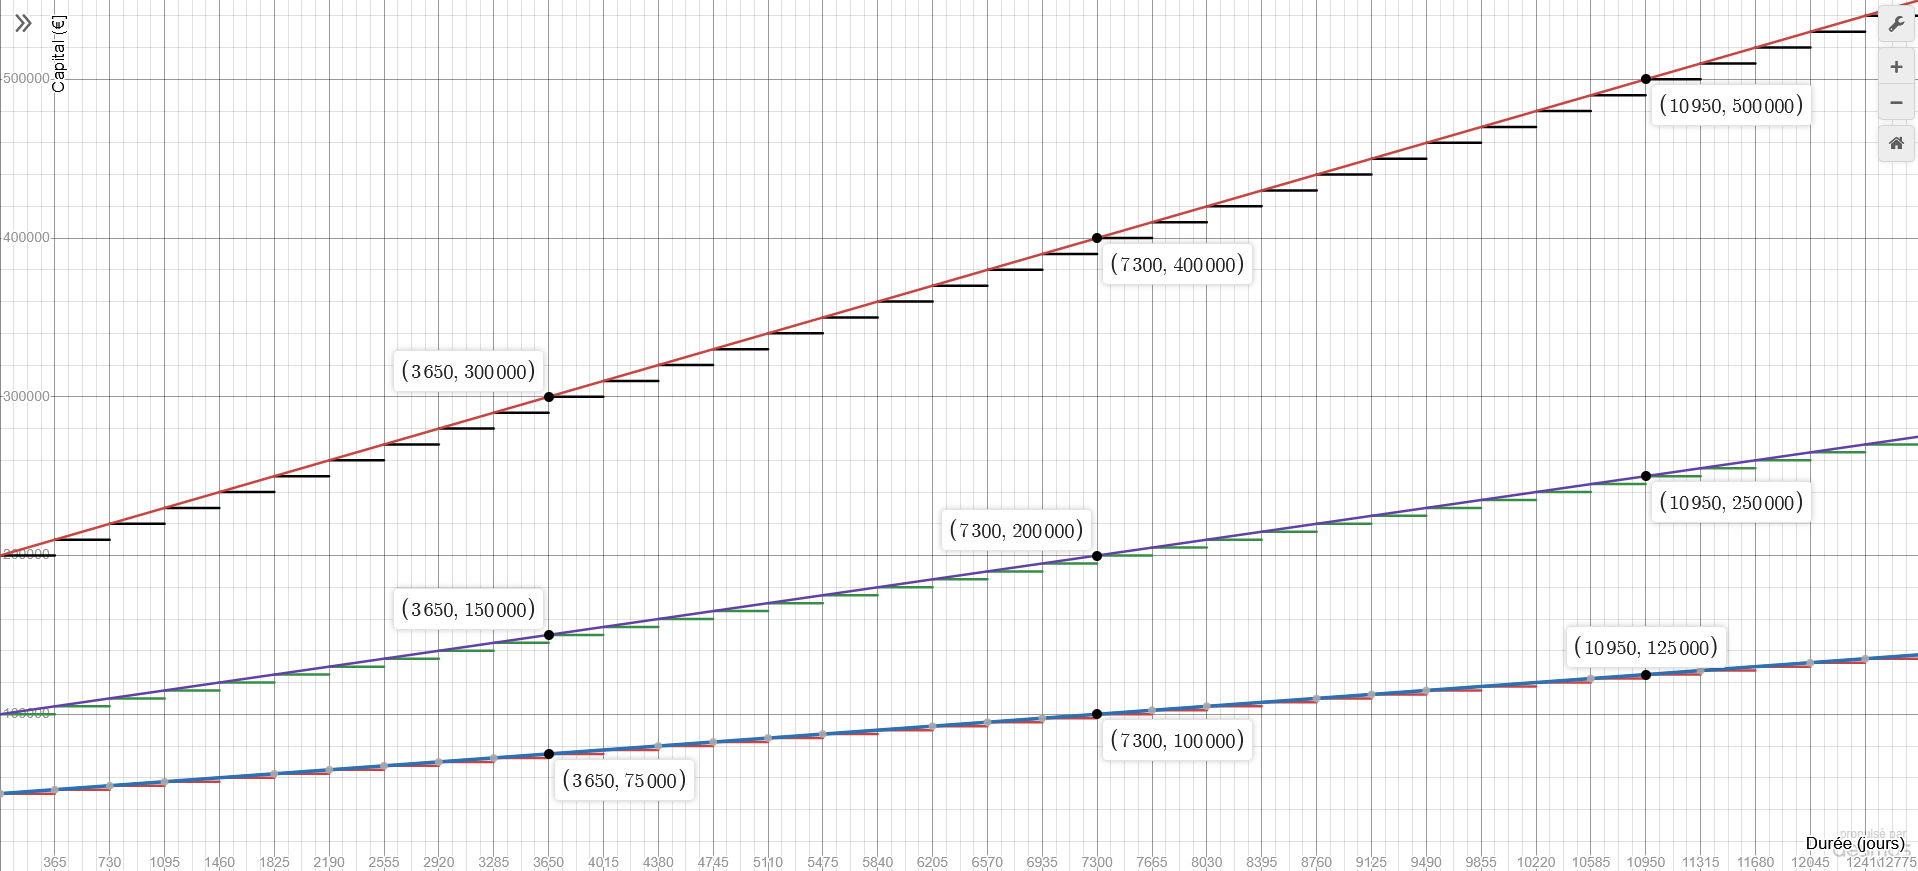
\includegraphics[width=1.35\textwidth]{lecture_graphique_interets_simples.png}}
	      	\caption{Lecture graphique du capital obtenu après 10, 20 et 30 ans d'investissement.}
	      	\label{fig:lecture_graphique_interets_simples}
	      \end{figure}
	      
	      % Exprimer le coefficient multiplicateur du capital initial en fonction de la durée d’investissement et du taux périodique.
	\item Le coefficient multiplicateur du capital initial, noté \( k(t) \), représente le facteur par lequel le capital initial est multiplié pour obtenir le capital final après une certaine durée d'investissement \( t \), avec un taux périodique \( r_q \) (taux d'intérêt par période). Ainsi, le coefficient multiplicateur \( k(t) \) est le rapport entre le capital final \( C(t) \) et le capital initial \( C_0 \) :
	      \[
	      	k(t) = \frac{C(t)}{C_0} = \frac{C_0 \left( 1 + r_q \cdot t \right)}{C_0} = 1 + r_q \cdot t = \boxed{1 + r_q \cdot t}
	      \]
	      
	      Vérification :
	      \begin{itemize}
	      	\item Pour 10 ans : $k(10) = 1 + 0,05 \times 10 = 1 + 0,5 = \boxed{1,5}$
	      	\item Pour 20 ans : $k(20) = 1 + 0,05 \times 20 = 1 + 1 = \boxed{2}$
	      	\item Pour 30 ans : $k(30) = 1 + 0,05 \times 30 = 1 + 2,5 = \boxed{2,5}$
	      \end{itemize}
	      
	\item Voir figure \ref{fig:coefficient_multiplicateur}.
	      \begin{figure}[h!]
	      	\centering
	      	\makebox[\textwidth][c]{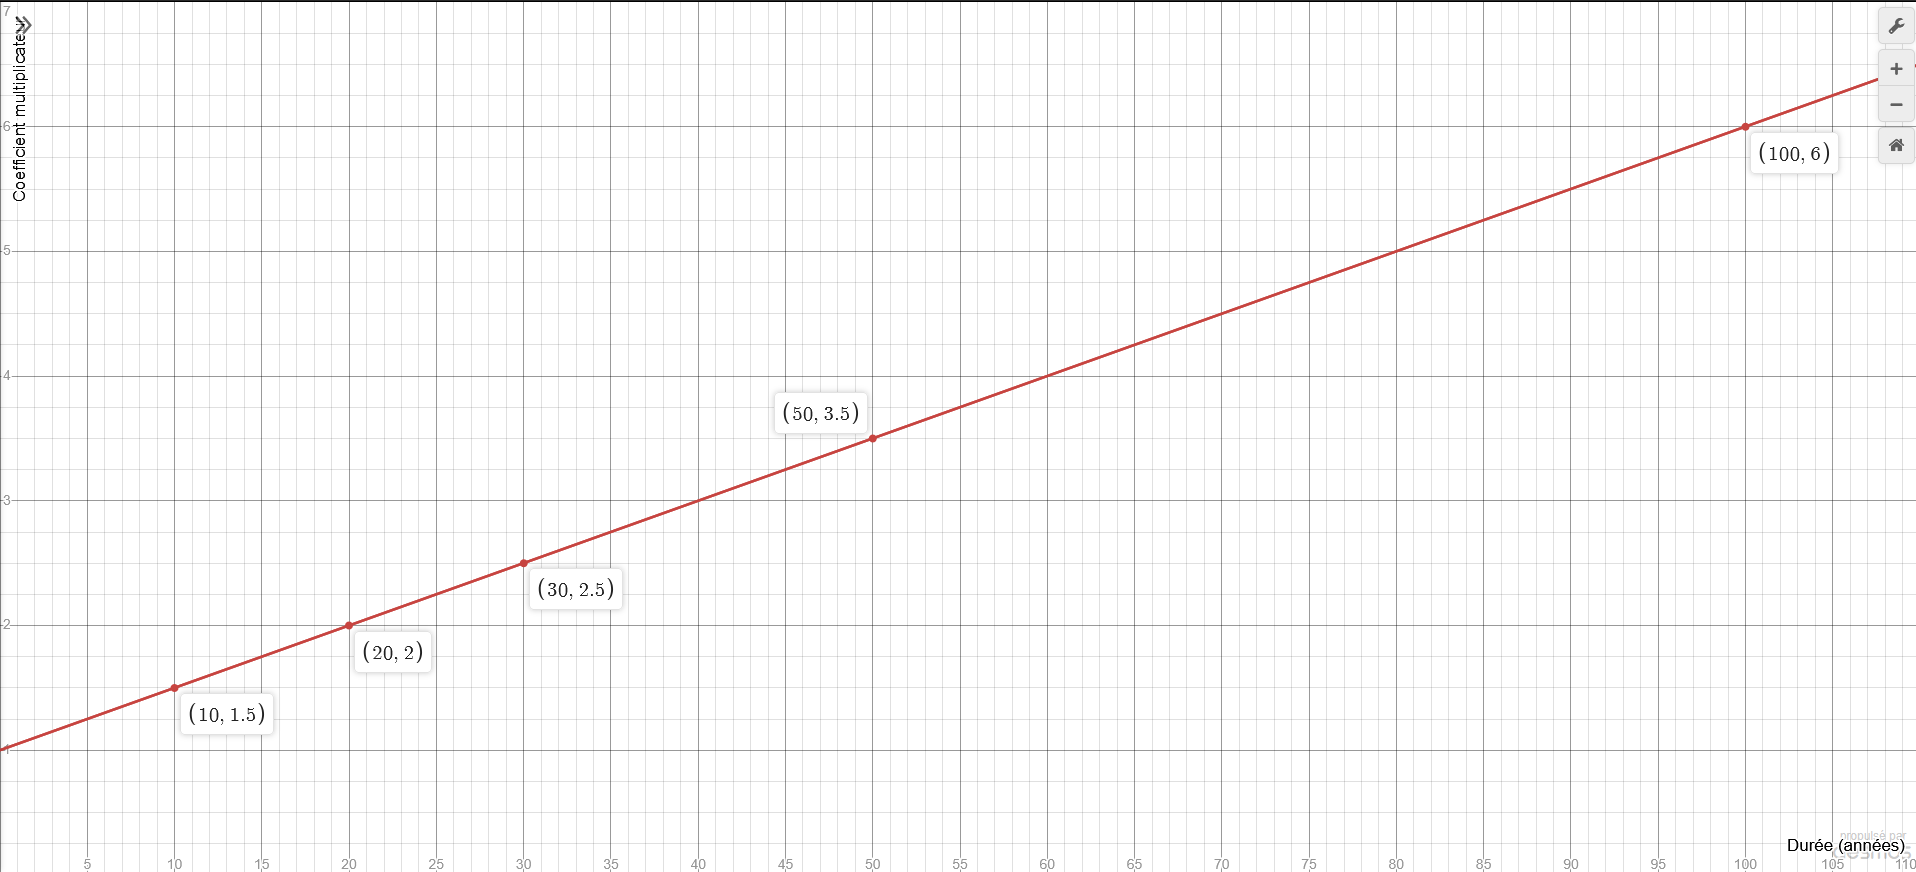
\includegraphics[width=1.35\textwidth]{coefficient_multiplicateur.png}}
	      	\caption{Coefficient multiplicateur du capital initial en fonction de la durée \( t \) (en années) pour un taux périodique de 5\% : \( k(t) = 1 + 0,05 \times t \)}
	      	\label{fig:coefficient_multiplicateur}
	      \end{figure}
	      
	      \begin{itemize}
	      	\item $k(10) = 1,5$
	      	\item $k(20) = 2$
	      	\item $k(30) = 2,5$
	      	\item $k(50) = 3,5$
	      	\item $k(100) = 6$
	      \end{itemize}
	      
	\item Pour un capital initial de \( 72\,924,\!56\ \text{€} \) à \( 5\,\% \) annuel en intérêts simples :
	      \begin{align*}
	      	C^s(10)  & = 72\,924,\!56 \times 1,\!5   = 109\,386,\!84\ \text{€} \\[0.4em]
	      	C^s(20)  & = 72\,924,\!56 \times 2,\!0   = 145\,849,\!12\ \text{€} \\[0.4em]
	      	C^s(30)  & = 72\,924,\!56 \times 2,\!5   = 182\,311,\!40\ \text{€} \\[0.4em]
	      	C^s(50)  & = 72\,924,\!56 \times 3,\!5   = 255\,235,\!96\ \text{€} \\[0.4em]
	      	C^s(100) & = 72\,924,\!56 \times 6,\!0   = 437\,547,\!36\ \text{€} 
	      \end{align*}
	      
	\item Étant donné la formule pour \( C_q^s(t) \) :
	      
	      \[
	      	C_q^s(t) = C_0 \times \left(1 + \frac{0{,}05}{365} \times t\right)\,,
	      \]
	      
	      \begin{itemize}
	      	\item Pour \( C_0 = 50\,000 \) € :
	      	      \[
	      	      	\begin{aligned}
	      	      		m & = \frac{C^s_q(1) - C^s_q(0)}{1 - 0}                                                                                                                 \\
	      	      		  & = \frac{50\,000 \times \left(1 + \frac{0{,}05}{365} \times 1\right) - 50\,000}{1}                                                                   \\
	      	      		  & \approx 50\,006{,}849 - 50\,000                                                                                                                     \\
	      	      		  & \approx 6{,}85\ \text{€}                                                                                                                          \\[1em]
	      	      		m & = \frac{C^s_q(1\,948) - C^s_q(32)}{1\,948 - 32}                                                                                                     \\
	      	      		  & = \frac{50\,000 \times \left(1 + \frac{0{,}05}{365} \times 1\,948\right) - 50\,000 \times \left(1 + \frac{0{,}05}{365} \times 32\right)}{1\,916}    \\
	      	      		  & \approx \frac{63\,342{,}46575 - 50\,219{,}17808}{1\,916}                                                                                            \\
	      	      		  & \approx \frac{13\,123{,}28767}{1\,916}                                                                                                              \\
	      	      		  & \approx 6{,}85\ \text{€}                                                                                                                          \\[1em]
	      	      		m & = \frac{C^s_q(365\,000) - C^s_q(364\,999)}{365\,000 - 364\,999}                                                                                     \\
	      	      		  & = \frac{50\,000 \times \left(1 + \frac{0{,}05}{365} \times 365\,000\right) - 50\,000 \times \left(1 + \frac{0{,}05}{365} \times 364\,999\right)}{1} \\
	      	      		  & \approx 2\,550\,000 - 2\,549\,993,15068                                                                                                             \\
	      	      		  & \approx 6{,}85\ \text{€}                                                                                                                          
	      	      	\end{aligned}
	      	      \]
	      	          
	      	\item Pour \( C_0 = 100\,000 \) € :
	      	      \[
	      	      	\begin{aligned}
	      	      		m & = \frac{C^s_q(1) - C^s_q(0)}{1 - 0}                                                                                                                   \\
	      	      		  & = \frac{100\,000 \times \left(1 + \frac{0{,}05}{365} \times 1\right) - 100\,000}{1}                                                                   \\
	      	      		  & \approx 100\,013{,}698 - 100\,000                                                                                                                     \\
	      	      		  & \approx 13{,}70\ \text{€}                                                                                                                           \\[1em]
	      	      		m & = \frac{C^s_q(1\,948) - C^s_q(32)}{1\,948 - 32}                                                                                                       \\
	      	      		  & = \frac{100\,000 \times \left(1 + \frac{0{,}05}{365} \times 1\,948\right) - 100\,000 \times \left(1 + \frac{0{,}05}{365} \times 32\right)}{1\,916}    \\
	      	      		  & \approx \frac{126\,684{,}9315 - 100\,438{,}35616}{1\,916}                                                                                             \\
	      	      		  & \approx \frac{26\,246{,}57534}{1\,916}                                                                                                                \\
	      	      		  & \approx 13{,}70\ \text{€}                                                                                                                           \\[1em]
	      	      		m & = \frac{C^s_q(365\,000) - C^s_q(364\,999)}{365\,000 - 364\,999}                                                                                       \\
	      	      		  & = \frac{100\,000 \times \left(1 + \frac{0{,}05}{365} \times 365\,000\right) - 100\,000 \times \left(1 + \frac{0{,}05}{365} \times 364\,999\right)}{1} \\
	      	      		  & \approx 5\,100\,000 - 5\,099\,986,30136                                                                                                               \\
	      	      		  & \approx 13{,}70\ \text{€}                                                                                                                           
	      	      	\end{aligned}
	      	      \]
	      	          
	      	\item Pour \( C_0 = 200\,000 \) € :
	      	      \[
	      	      	\begin{aligned}
	      	      		m & = \frac{C^s_q(1) - C^s_q(0)}{1 - 0}                                                                                                                   \\
	      	      		  & = \frac{200\,000 \times \left(1 + \frac{0{,}05}{365} \times 1\right) - 200\,000}{1}                                                                   \\
	      	      		  & \approx 200\,027{,}397 - 200\,000                                                                                                                     \\
	      	      		  & \approx 27{,}40\ \text{€}                                                                                                                           \\[1em]
	      	      		m & = \frac{C^s_q(1\,948) - C^s_q(32)}{1\,948 - 32}                                                                                                       \\
	      	      		  & = \frac{200\,000 \times \left(1 + \frac{0{,}05}{365} \times 1\,948\right) - 200\,000 \times \left(1 + \frac{0{,}05}{365} \times 32\right)}{1\,916}    \\
	      	      		  & \approx \frac{253\,369{,}863 - 200\,876{,}71232}{1\,916}                                                                                              \\
	      	      		  & \approx \frac{52\,493{,}15068}{1\,916}                                                                                                                \\
	      	      		  & \approx 27{,}40\ \text{€}                                                                                                                           \\[1em]
	      	      		m & = \frac{C^s_q(365\,000) - C^s_q(364\,999)}{365\,000 - 364\,999}                                                                                       \\
	      	      		  & = \frac{200\,000 \times \left(1 + \frac{0{,}05}{365} \times 365\,000\right) - 200\,000 \times \left(1 + \frac{0{,}05}{365} \times 364\,999\right)}{1} \\
	      	      		  & \approx 10\,200\,000 - 10\,199\,972,60272                                                                                                             \\
	      	      		  & \approx 27{,}40\ \text{€}                                                                                                                           
	      	      	\end{aligned}
	      	      \]
	      \end{itemize}
	      
	\item Le coefficient directeur représente le montant des intérêts gagnés chaque jour.
	      
	\item Le coefficient directeur \( m \) d'une droite entre deux points \((x_a, C_q^s(x_a))\) et \((x_b, C_q^s(x_b))\) est donné par :
	          
	      \[
	      	m = \frac{C_q^s(x_b) - C_q^s(x_a)}{x_b - x_a}
	      \]
	          
	      La fonction \( C_q^s(t) \) est définie comme :
	          
	      \[
	      	C_q^s(t) = C_0 \times \left(1 + r \times t\right)
	      \]
	              
	      Substitution de \( C_q^s(x_b) \) et \( C_q^s(x_a) \) dans la formule du coefficient directeur :
	          
	      \[
	      	m = \frac{C_0 \times \left(1 + r \times x_b\right) - C_0 \times \left(1 + r \times x_a\right)}{x_b - x_a}
	      \]
	          
	      Développement des termes du numérateur selon l'identité $a \times (b + c) = a \times b + a \times c$ :
	      
	      \[
	      	m = \frac{\overset{a}{\overbrace{C_0}} \times (\overset{b}{\overbrace{1}} + \overset{c}{\overbrace{r \times x_b}}) - C_0 \times (1 + r \times x_a)}{x_b - x_a}
	      \]
	      
	      \[
	      	m = \frac{C_0 + C_0 \times r \times x_b - \overset{a}{\overbrace{C_0}} \times (\overset{b}{\overbrace{1}} + \overset{c}{\overbrace{r \times x_a}})}{x_b - x_a}
	      \]
	          
	      \[
	      	m = \frac{C_0 + C_0 \times r \times x_b - C_0 - C_0 \times r \times x_a}{x_b - x_a}
	      \]
	          
	      Les termes \( C_0 \) sont constants et s'annulent :
	      
	      \[
	      	m = \frac{\cancel{C_0} + C_0 \times r \times x_b \cancel{- C_0} - C_0 \times r \times x_a}{x_b - x_a}
	      \]
	          
	      \[
	      	m = \frac{C_0 \times r \times x_b - C_0 \times r \times x_a}{x_b - x_a}
	      \]
	          
	      Factorisation de $(C_0 \times r)$ selon l'identité $a \times b - a \times c = a \times (b-c)$ :
	      
	      \[
	      	m = \frac{\overset{a}{\overbrace{C_0 \times r}} \times \overset{b}{\overbrace{x_b}} - \overset{a}{\overbrace{C_0 \times r}} \times \overset{c}{\overbrace{x_a}}}{x_b - x_a}
	      \]
	          
	      \[
	      	m = \frac{\overset{a}{\overbrace{C_0 \times r}} \times (\overset{b}{\overbrace{x_b}} - \overset{c}{\overbrace{x_a}})}{x_b - x_a}
	      \]
	      
	      \[
	      	m = C_0 \times r \times \frac{x_b - x_a}{x_b - x_a}
	      \]
	          
	      Puisque $\frac{x_b - x_a}{x_b - x_a} = 1$ pour $x_b - x_a \neq 0$ :
	      \[
	      	\boxed{m = C_0 \times r}
	      \]
	          
	      Le coefficient directeur \( m \) est donc constant et égal à \( C_0 \times r \), où \( r \) est le rendement périodique quotidien. Cela montre que le coefficient directeur est proportionnel au capital initial et au rendement périodique, indépendamment des points \( x_a \) et \( x_b \) choisis.
	      
	\item Le coefficient directeur constant traduit une croissance linéaire du capital dû au versement des intérêts d'un montant fixe. Graphiquement, la fonction forme une droite, avec une pente représentant le gain périodique. Cette linéarité garantit une prévisibilité totale, mais limite la rentabilité sur le long terme (pas d’effet de capitalisation).
	      
	\item Exemples de dispositifs avec des intérêts simples :
	      \begin{itemize}
	      	\item Crédit immobilier ou à la consommation (les intérêts  sont calculés sur le capital restant dû).
	      	\item Obligation à taux fixe sans réinvestissement des coupons.
	      \end{itemize}
	      
	\item En période d'inflation, les intérêts perdent de la valeur réelle car le montant est grignoté par la hausse globale des prix. À l’inverse, en déflation, ces mêmes intérêts gagnent en pouvoir d’achat grâce à la baisse générale des prix. 
	      
	      La BCE vise une inflation cible de \( 2\% \), un équilibre permettant d’éviter les excès déflationnistes tout en limitant l’érosion des rendements. Cependant, même une inflation modérée agit avec un effet boule de neige : l’augmentation lente mais cumulée des prix, année après année, ronge progressivement la valeur réelle des intérêts simples, dont le montant reste constant.
	      
	\item Lorsque les intérêts générés sont réinvestis dans un actif financier, ils produisent à leur tour des intérêts. Ce mécanisme, appelé capitalisation des intérêts ou intérêts composés, consiste à incorporer les gains au capital initial, ce qui augmente progressivement la base de calcul des futurs intérêts et engendre une croissance exponentielle du rendement.
\end{enumerate}

\end{document}
